\documentclass[10pt,conference,compsocconf]{IEEEtran}
\documentclass[10pt,conference]{IEEEtran}

\usepackage{hyperref}
\usepackage{graphicx}
\usepackage{booktabs}
\usepackage{amsmath}
\hypersetup{hidelinks}

\begin{document}
\title{Predicting Coronary Heart Disease from BRFSS Survey Answers with Regularized Logistic Regression}

\author{
  Antonin Hocquet, David Attias, Ivan Pouly\\
  \textit{CS-433 Machine Learning, EPFL, Switzerland}
}

\maketitle

\begin{abstract}
The Behavioral Risk Factor Surveillance System (BRFSS) collects state data about U.S. residents regarding their health-related risk behaviors, chronic health conditions, and use of preventive services. The data is collected via telephone surveys. We predict the presence of a coronary heart disease or a heart attack in the respondents of 2015 BRFSS reports, by applying the ridge regression and the L2-regularized logistic regression. We reach the score of $F_1 = 0.429 \pm 0.005$ in 5-fold cross-validation and $0.437$ on the AIcrowd test set. \cite{aicrowd2026}. Our preprocessing reduces the initial 321 features of the data to 76, from which we create the 488 features of our design matrix. The effect of our different methods to the F1 score is the following : logistic loss instead of the square loss added $0.009$ to our F1 score and adding the interactions of the features with age added $0.002$. Adding further features did not change F1 by more than $0.001$.
\end{abstract}

\section{Introduction}
The training set contains the answers of 328{,}135 respondents, which are described by 321 variables (see \cite{brfss2015}). Each respondent receives a binary label that represents whether they reported having been told by a provider they had a coronary heart disease. The test set contains 109{,}379 respondents. Only 8.8\% of the training respondents are positive. To rank our predictions, we use the $F_1$ score which is given by the harmonic mean of the precision (the probability that someone predicted positive is positive) and the recall (the probability that someone positive is predicted positive).


\section{Evaluation protocol}
We use 5-fold cross-validation (CV) on one fixed random split (seed 1). The scores are reported as the mean scores over the fold $\pm$ the standard deviation over the folds. The paired effects are reported as the mean difference $\pm$ standard deviation. The preprocessing is done after the cross-validations, so that the transformations applied to the raw data depends only on the training fold. Similarly, the decision threshold maximising $F_1$ is chosen only over the training folds.


\section{Data preprocessing}
We used the Centers for Disease Control and Prevention (CDC) codebook and calculated-variable documentation~\cite{brfss2015,brfsscv2015} and we kept only 73 raw variables of the 321 available. We removed record identifiers and interview logistics (e.g.\ \texttt{SEQNO}, \texttt{FMONTH}), phone-screening questions that are constant among respondents, survey weights, raw answers duplicated by a cleaner CDC calculated variable (e.g.\ \texttt{WTKG3} replaces \texttt{WEIGHT2}, which mixes pounds and kilograms), and the 109 optional-module questions, which are only asked in some states.

In particular, we removed the variable \texttt{HAREHAB1}, since it was the answer to the question ``Did you go to cardiac rehabilitation after your heart attack?''. All 773 respondents who answered it are positive (2.7\% of the positives). This is a leakage of the label, and because it makes no sense to predict a label from its leakage, we removed it.

Depending on the variable, ``don't know'' and ``refused'' codes (7/9, 77/99, \ldots) become missing, ``none'' (88) becomes 0, out-of-range sentinels (e.g.\ 900 and 99{,}900 in the alcohol variables) become missing, and heavy-tailed quantities (alcohol, fruit and vegetable intake, minutes of physical activity) are transformed by applying $\log(1+x)$.

We introduced 2 new variables : \texttt{IS\_PARTIAL} is an indicator that marks interviews that stopped before the end (15\% of rows); \texttt{HH\_ADULTS} merges the landline and cell-phone versions of the number of adults in the household.

For the 21 numeric or ordinal variables, we replaced the missing values with the median of the values we got. The 55 categorical variables are one-hot encoded. The missing values are replaced with the level that was the most frequent in the values we got. For each variable with at least 0.5\% missing values, we have added a missing-value indicator (57 indicators). We removed columns with more than 95\% of missing values. Finally, all the 244 columns are standardized.

To go further, after having standardized the age, we added the product of the standardized age with every other feature, and standardized again, so we got $487$ features, plus the intercept.


\section{Models}
As baselines we use the constant classifier (everybody is negative) and ridge regression (least squares with regularization parameter $\lambda = 3\cdot10^{-3}$ chosen by CV, we then output positive if and only if the output of the prediction by the ridge regression is at least $0.22$).

We minimize
\begin{equation}
\frac{1}{N}\sum_{n=1}^{N}\Big[\log\big(1+e^{x_n^\top w}\big)-y_n x_n^\top w\Big] + \frac{\lambda}{2}\lVert w_{1:}\rVert^2.
\end{equation}
We leave the intercept term $w_0$ unpenalized. We apply Newton's method: $w \leftarrow w - H^{-1}\nabla$, where $H = X^\top S X / N + \lambda I'$ and $S = \mathrm{diag}\big(p_n(1-p_n)\big)$. It converges in about ten iterations (stopping when $\max|\Delta w| < 10^{-6}$).

We select $\lambda \in \{10^{-2}, 10^{-3}, 10^{-4}, 10^{-5}\}$ by taking the $\lambda$ that maximizes the mean of the F1 scores over all testing folds ($\lambda = 10^{-4}$). Each time we choose a testing fold, we use the other folds as training folds. They then give us some predictions for the testing fold, with $\lambda = 10^{-4}$. We group these predictions over all testing folds to give us a prediction for each sample. Then, we choose the threshold $t = 0.205$ that maximizes $F_1$ on all these predictions. (Fig.~\ref{fig:threshold}).

We also tried sex~$\times$~feature interactions, a one-hot \texttt{GENHLTH}, and presence indicators of the module questions (Table~\ref{tab:ablation}).


\section{Results}
Table~\ref{tab:main} gives us the F1 scores for the different models we have tested and Table~\ref{tab:ablation} gives us the paired effect of each change we tested. We tried several combinations of the two missing-value thresholds (drop a variable above 40--95\% missing, add an indicator above 0, 0.5, 5 or 20\% missing, or never), the logistic model without age interactions stays between 0.425 and 0.428. We also tried adding squares and products of numeric variables and it did not help either (the F1 score stayed between $0.426$ and $0.427$).

\begin{table}[t]
\centering
\caption{5-fold CV $F_1$ (mean $\pm$ std over folds). Each indented row adds one change to the row above.}
\label{tab:main}
\begin{tabular}{lc}
\toprule
Model & CV $F_1$ \\
\midrule
Constant ``healthy'' (accuracy 0.912) & 0 \\
Ridge regression, 244 features & $0.418 \pm 0.005$ \\
Logistic regression (Newton), $\lambda=10^{-3}$ & $0.427 \pm 0.004$ \\
\quad + age interactions, $\lambda=10^{-4}$ (final) & $\mathbf{0.429 \pm 0.005}$ \\
\midrule
Final model, AIcrowd test set & 0.437 \\
\bottomrule
\end{tabular}
\end{table}


\begin{table}[t]
\centering
\caption{Paired effect on CV $F_1$ of each change to the final model (mean $\pm$ standard error over the 5 folds).}
\label{tab:ablation}
\begin{tabular}{lc}
\toprule
Change & $\Delta F_1$ \\
\midrule
No missing-value indicator & $-0.0007 \pm 0.0002$ \\
All indicators, drop variables ${>}65\%$ missing & $-0.0009 \pm 0.0003$ \\
\texttt{GENHLTH} one-hot instead of ordinal & $-0.0015 \pm 0.0009$ \\
+ 98--99 module-presence indicators & $+0.0004 \pm 0.0007$ \\
+ sex $\times$ feature interactions & $+0.0002 \pm 0.0009$ \\
\midrule
+ \texttt{HAREHAB1} presence (leak, excluded) & $+0.0082 \pm 0.0005$ \\
\bottomrule
\end{tabular}
\end{table}


\begin{figure}[t]
\centering
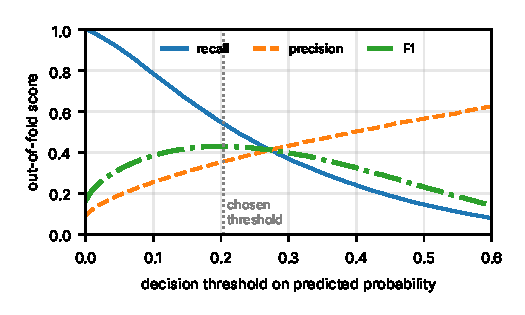
\includegraphics[width=\columnwidth]{threshold}
\caption{Out-of-fold recall, precision and $F_1$ of the final model against the decision threshold. $F_1$ peaks at $t = 0.205$, far below 0.5.}
\label{fig:threshold}
\end{figure}


\section{Discussion}
Three findings stand out. First, the loss matters more than the features: ridge regression fits the 0/1 labels with a squared loss and is clearly beaten by the logistic loss ($+0.009$), which models probabilities directly. Second, every step beyond the basic cleaning changed $F_1$ by $0.002$ or less, so the extra features brought little to the F1 score. Third, the F1-optimal threshold is low (Fig.~\ref{fig:threshold}). The final model flags 13.4\% of the respondents and finds 55\% of the positives with a precision of 36\%.

The test score (0.437) is 0.008 above our F1 measured with CV. With about 9{,}700 positives expected in the test set, the gap is due to the randomness of the sample chosen for the test set.

\section{Summary}
We chose only 73 raw variables from the 321 available, we encoded them into 488 features which we normalized. The only interaction between variables we added was the relation between age and all the other variables. We applied an L2-regularized logistic regression with Newton's method to give $F_1 = 0.429$ in CV and $0.437$ on the test set. The file \texttt{run.py} reproduces the submission in a few minutes, \texttt{model\_search.py} repeats the selection of $\lambda$ and of the threshold, and \texttt{ablations.py} reproduces Tables~\ref{tab:main} and~\ref{tab:ablation}.

\bibliographystyle{IEEEtran}
\bibliography{literature}

\end{document}
